\chapter{Prevalence modelling and regression methods}

\textcite[p. 311]{fisher1922mathematical} stated that the objective of
statistics is to reduce the data since its volume is impossible 
to comprehend by the researchers. In that sense, few parameters should represent the whole phenomenon catching the most relevant information. 
Years later, Newman studied the theory of modelling which can be divided 
in three aspects \cite[p. 161]{lehmann2012model}: 

\begin{enumerate}
  \item models of complex phenomena are created by putting together 
  simple building elements that the researcher is familiar with and can 
  handle; 
  \item there are two types of models: the \textit{explanatory models}, 
  which will be focused on this work, and the \textit{interpolatory formulae}. 
  \item An explanatory theory necessitates a thorough understanding of the scientific context of the problem. In this regard, we investigated questions involving Respondent-driven sampling and prevalence estimation as introduced in Chapter \ref{ch:theoretical-background}. 
\end{enumerate}

In this chapter, we develop models that enclose these ideas building each 
block separately. For a Bayesian modelling, we assume that each parameter
of the model has a probability distribution that incorporates the 
researcher's uncertainty about it. For each individual, we observe $k$ 
covariates that are possible risk factors represented by the vector 
$\x_i \in \R^{k}$ of the $i^{th}$ individual. We denote $\theta_i$ the 
probability of the $i$-th individual have been exposed to the disease
that depends on the prevalence $\theta$ and $\x_i$. We also consider the
dependence of sampling from RDS as a spatial random effect. The probability of
positive test in the $i^{th}$ individual is denoted by $p_i$.  

Another important feature of the model is that sensitivity and 
specificity have the same distribution for all individuals and 
it only depends on the test used to diagnose. This is an assumption 
that must be analysed for each particular case. For instance, COVID-19 
Sofia test has different sensibility and specificity for symptomatic and 
asymptomatic individuals \cite[Table 1][p. 3]{mitchell2021performance}.  

From above, we develop three different models: the first considers perfect 
tests, that is, $\gamma_s = \gamma_e = 1$ and no spatial random effect; 
the second considers imperfect tests, regarding $\gamma_s$ and $\gamma_e$, 
but ignoring the RDS structure; and the third one has imperfect tests and 
RDS structure. \improve{Some considerations are made to improve the model's
limitations.}

The implementation of the following models were in the statistical computation
platform Stan \cite{carpenter2017stan} within Python Interface PyStan
\cite{pystan} which uses an implementation for HMC algorithm. All the codes
are written in \autoref{appendix:stan-codes}.

\section{Perfect tests}

The first model supposes the samples are independent and the test is perfect,
which means that $\theta_i = p_i$ for all $i$. Therefore it only considers the risk factors $\x_i$. 

\begin{equation}
  \begin{aligned}
    Y_i \mid \theta_i &\sim \bern(\theta_i), \\
    g(\theta_i) &= g(\theta) + \x_i^T\beta, 
  \end{aligned}  
\end{equation}
where $g(\cdot)$ is the $\operatorname{logit}$ function.
The parameter $\beta \in \R^{k}$ is the risk effects. For Bayesian inference, priors on
$\beta$ and $\theta$ must be included. We use $\beta ~ \sim \N(\mu_{\beta}, \Sigma_{\beta})$
and $\theta \sim \betadist(a^{p}, b^p)$, where the vector $\mu_{\beta}
\in \R^{k}$, the symmetric positive-definite matrix $\Sigma_{\beta} \in
\R^{k\times k}$, and the positive real values $a^p, b^p \in \R_{>0}$ are fixed
hyperparameters. Inferences about $\beta$ and $\theta$ are based on the posterior distribution.

If the risk factors are zero, i.e $\x_i = 0$, the probability of the
$i$-th individual having been exposed is the prevalence $\theta$, which means that in
a population with no risk effects, the probability of a person having the
disease is exactly the proportion in this population. Keeping the notation of
Section \ref{sec:glm}, we denote $\boldsymbol{X}$ the covariate matrix. 

\subsection{Identifiability}

Identifiability is characterized by the likelihood function. In our model, if
given data points $y$, two different values of $\theta$ yield the
same likelihood function, then $\theta$ is {\em unidentifiable}. The same for
each $\beta_i$. In this circunstancies, proper priors are sufficient to handle
identifiability problems in Bayesian perspective \cite[p.
3459]{xie2006measures}. A formal definition for {\em Bayesian identifiability}
is the following: if $p(\theta \mid \beta, y, \boldsymbol{X}) = p(\theta \mid
\beta)$, the
data $y$ is uninformative for $\theta$ when $\beta$ is known. We can change
the places of $\beta$ and $\theta$ with the same definition. 



"if the observed values of x i are “far from” zero, resulting
in potentially strong posterior correlation among b 0 and
b 1 (see Fig. 2). To address this problem, centering of x i" (ogle, 2020). 

\subsection{Simulated data}

To present a sanity check about the functionality of the above model, we
generate simulated data from the model and make inferences about the result. 

\section{Sensitivity and specificity}

In this section, we describe a model for estimating the sensitivity and
specificity of a diagnostic test separately from the final model for
estimating prevalence. This model is relevant to analyze and experiment with
different prior specification approaches. Suppose having a {\em gold standard
test} that is the best available test \cite{versi1992gold}, and also another
test (for instance a simpler, a faster, or a less invasive one) which we want
to estimate the accuracy by the sensitivity and specificity. In this scenario,
a true positive / negative individual means they have been tested positive by
the gold standard. Therefore, in a population with $n_{\gamma_e}$ true
positives and  $n_{\gamma_s}$ true negatives, we denote 
\begin{gather*}
  y_{negative} \sim \operatorname{Binomial}(n_{\gamma_e}, \gamma_e), \\
  y_{positive} \sim \operatorname{Binomial}(n_{\gamma_s}, \gamma_s),
\end{gather*}
such that $y_{negative}$ are negative tests on known negative 
subjects and $y_{positive}$ are positive tests on
known positive. In a classic Bayesian analysis, we have to define a 
prior distribution for the parameters $(\gamma_e, \gamma_s) \sim \pi(\gamma_e,
\gamma_s)$. 

For this, we consider three different approaches: 

\begin{enumerate}
  \item The parameters are independent a priori and each one has a beta
  distribution with pre-specified hyperparameters.
  \item \improve{Hierarchical partial pooling, when dealing with more studies.}
  \item A Bivariate Beta (see Appendix
  \ref{appendix:bivariate-beta-distribution}) 
  distribution.
\end{enumerate}

\subsection{Independent beta distribution priors}

When considering separated experiments for specificity and
sensitivity, there is
no information about their correlation, which is the case for our model. Then we define the the prior distributions
\begin{gather*}
  \gamma_e \sim \operatorname{Beta}(a_e, b_e), \\
  \gamma_s \sim \operatorname{Beta}(a_s, b_s), \\
  \theta \sim \operatorname{Beta}(a_{\theta}, b_{\theta}).
\end{gather*} 
Using data from \cite{bennett2020estimating} about COVIDPrior information of these quantities lead to a bivariate analysis {cite:t}`guo2017bayesian`. As we have already mentioned, the definitions of *sensitivity* and
*specificity* can be expressed as below: -19 seroprevalence in
Santa Clara:  
\begin{align*}
  y/n &= 50/3330,\\
y_{negative}/n_{\gamma_e} &= 399/401, \\
y_{positive}/n_{\gamma_s} &= 103/122, 
\end{align*}
we fit the model and obtain the results showed in Figure
\ref{fig:results-posterior-model1}. All the codes were done in {\em Stan} and
{\em PyStan}.

\begin{figure}[!ht]
  \centering
  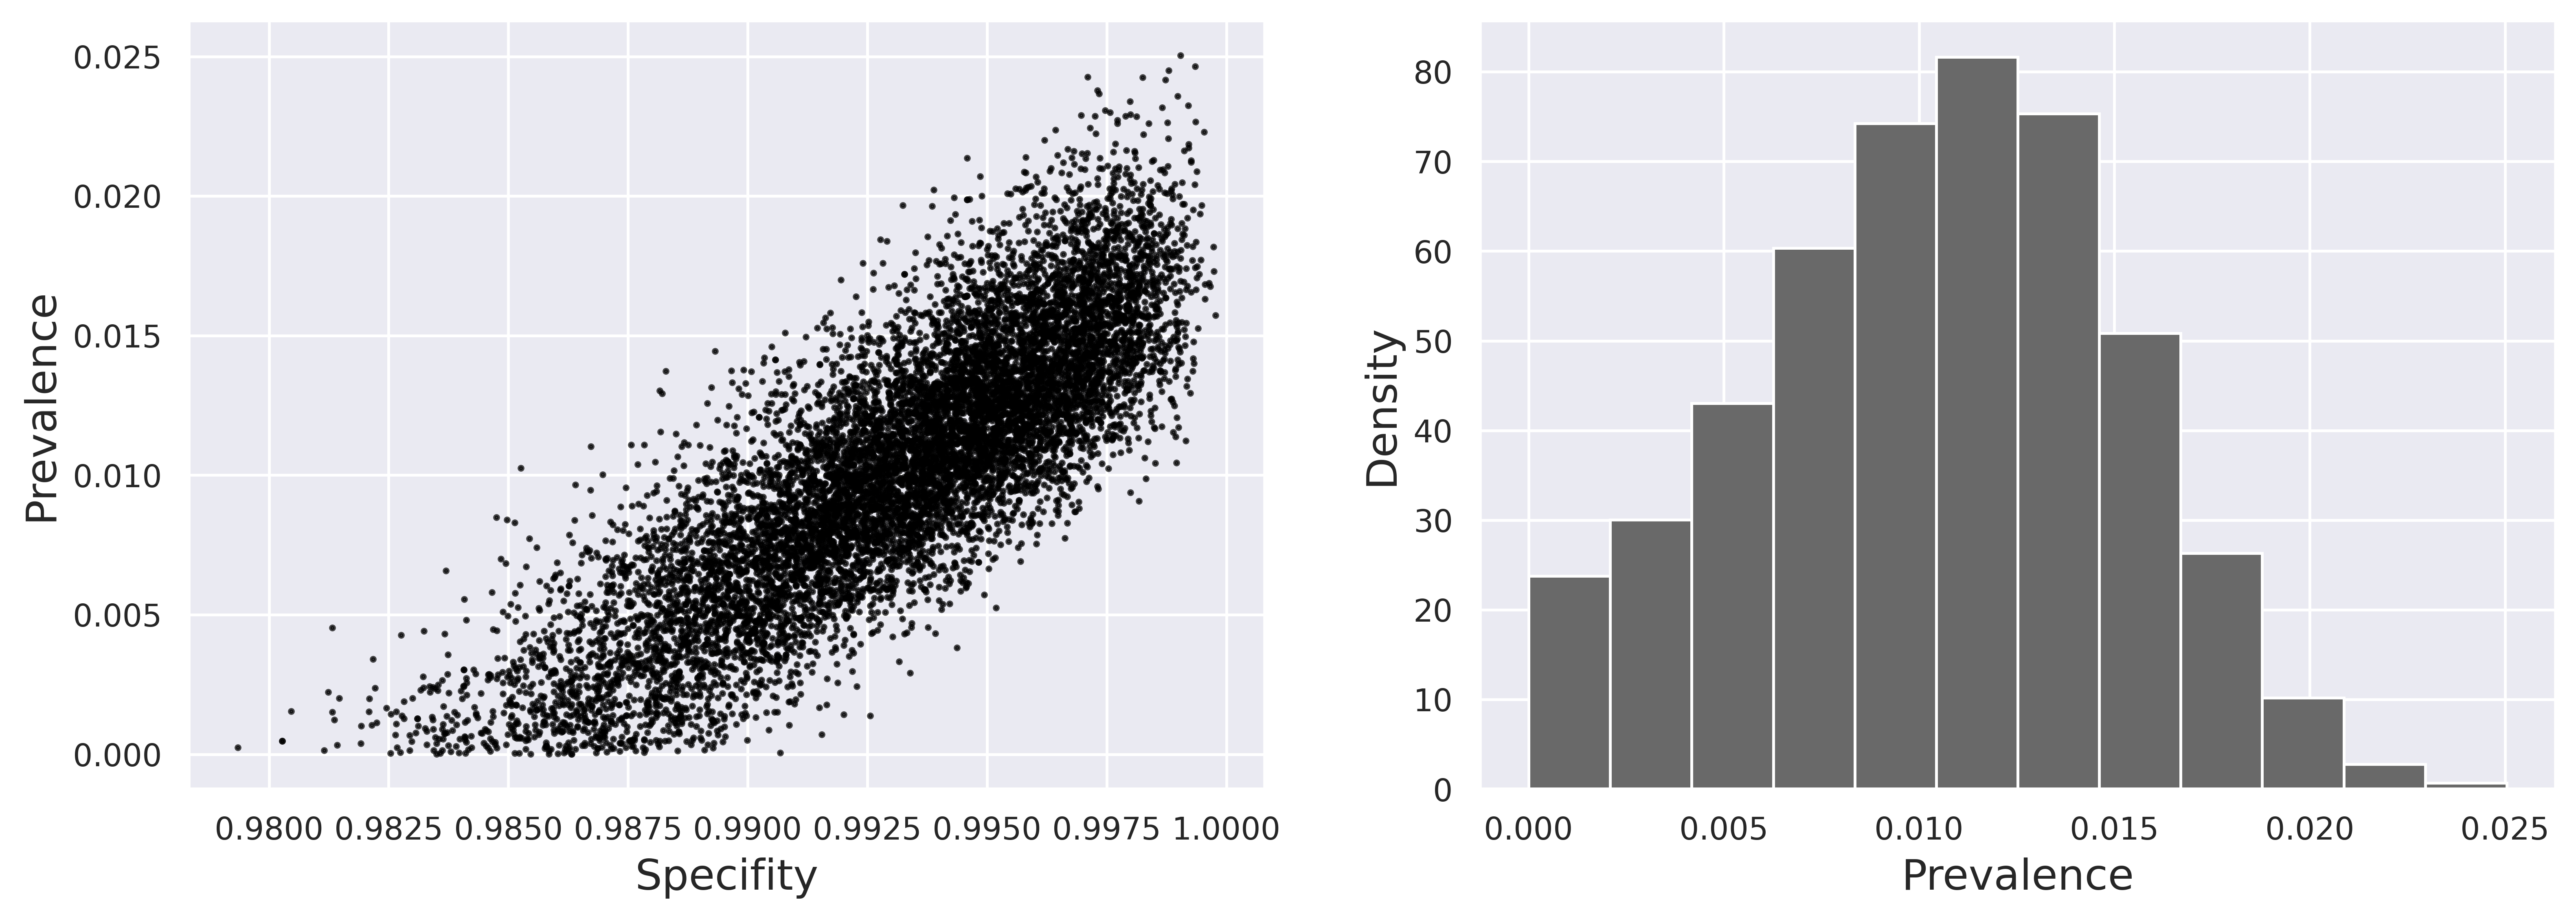
\includegraphics[width=\textwidth]{../../images/model1_gelman_figure_english.png}
  \caption{Scatter plot of posterior simulations of prevalence against
  specificity and histogram of posterior simulations of the prevalence.}
  \label{fig:results-posterior-model1}
\end{figure}

\subsection{Hierarchical partial pooling prior}

Other approach considers more than one study about specificity and
sensitivity. A {\em hierarchical partial pooling} model for these studies
can be done in the following way: 
\begin{gather*}
    \operatorname{logit}(\gamma_s^j) \sim \operatorname{Normal}(\mu_{\gamma_s}, \sigma_{\gamma_s}), \\
    \operatorname{logit}(\gamma_e^j) \sim \operatorname{Normal}(\mu_{\gamma_e}, \sigma_{\gamma_e}), 
\end{gather*}
for $1 \le j \le K$ studies, such that the first study is the considered one.
Partial pooling because the parameters can be sampled from the same
distribution. Hierarchical because the parameters of this distribution have
its one prior distributions. For instance, 
\begin{align*}
    \mu_{\gamma_s} &\sim N(0, 10), \\ 
    \mu_{\gamma_e} &\sim N(0, 10), \\
    \sigma_{\gamma_s} &\sim N^+(0,1), \text{ and } \\
    \sigma_{\gamma_e} &\sim N^+(0,1),
\end{align*}
where $N^+(a,b)$ is the truncated normal distribution in $[0,+\infty)$.

\subsection{Bivariate Beta prior}

Finally, we studied a joint distribution for specificity and sensitivity, a
possible bivariate beta distribution built in \cite{olkin2015constructions}.
This distribution is derived from a Dirichlet distribution of order four. Let $U = (U[1],...,U[4]) \sim \operatorname{Dirichlet}(\boldsymbol{\alpha})$, where
$\boldsymbol{\alpha} \in \mathbb{R}^4_+$. Therefore, defining $X = U[1] +
U[2]$ and $Y = U[1] + U[3]$, we will have that $(X,Y)$ has a well-defined
probability distribution in
$[0,1] \times [0,1]$ such that $X$ and $Y$ have marginally beta distributions,
and they have correlation in all space. Depending on the definition of
$\boldsymbol{\alpha}$, the correlation between the variables range from -1 and
1. Figure \ref{fig:beta-bivariate} shows some examples of this construction. 

\begin{figure}[!ht]
    \centering
    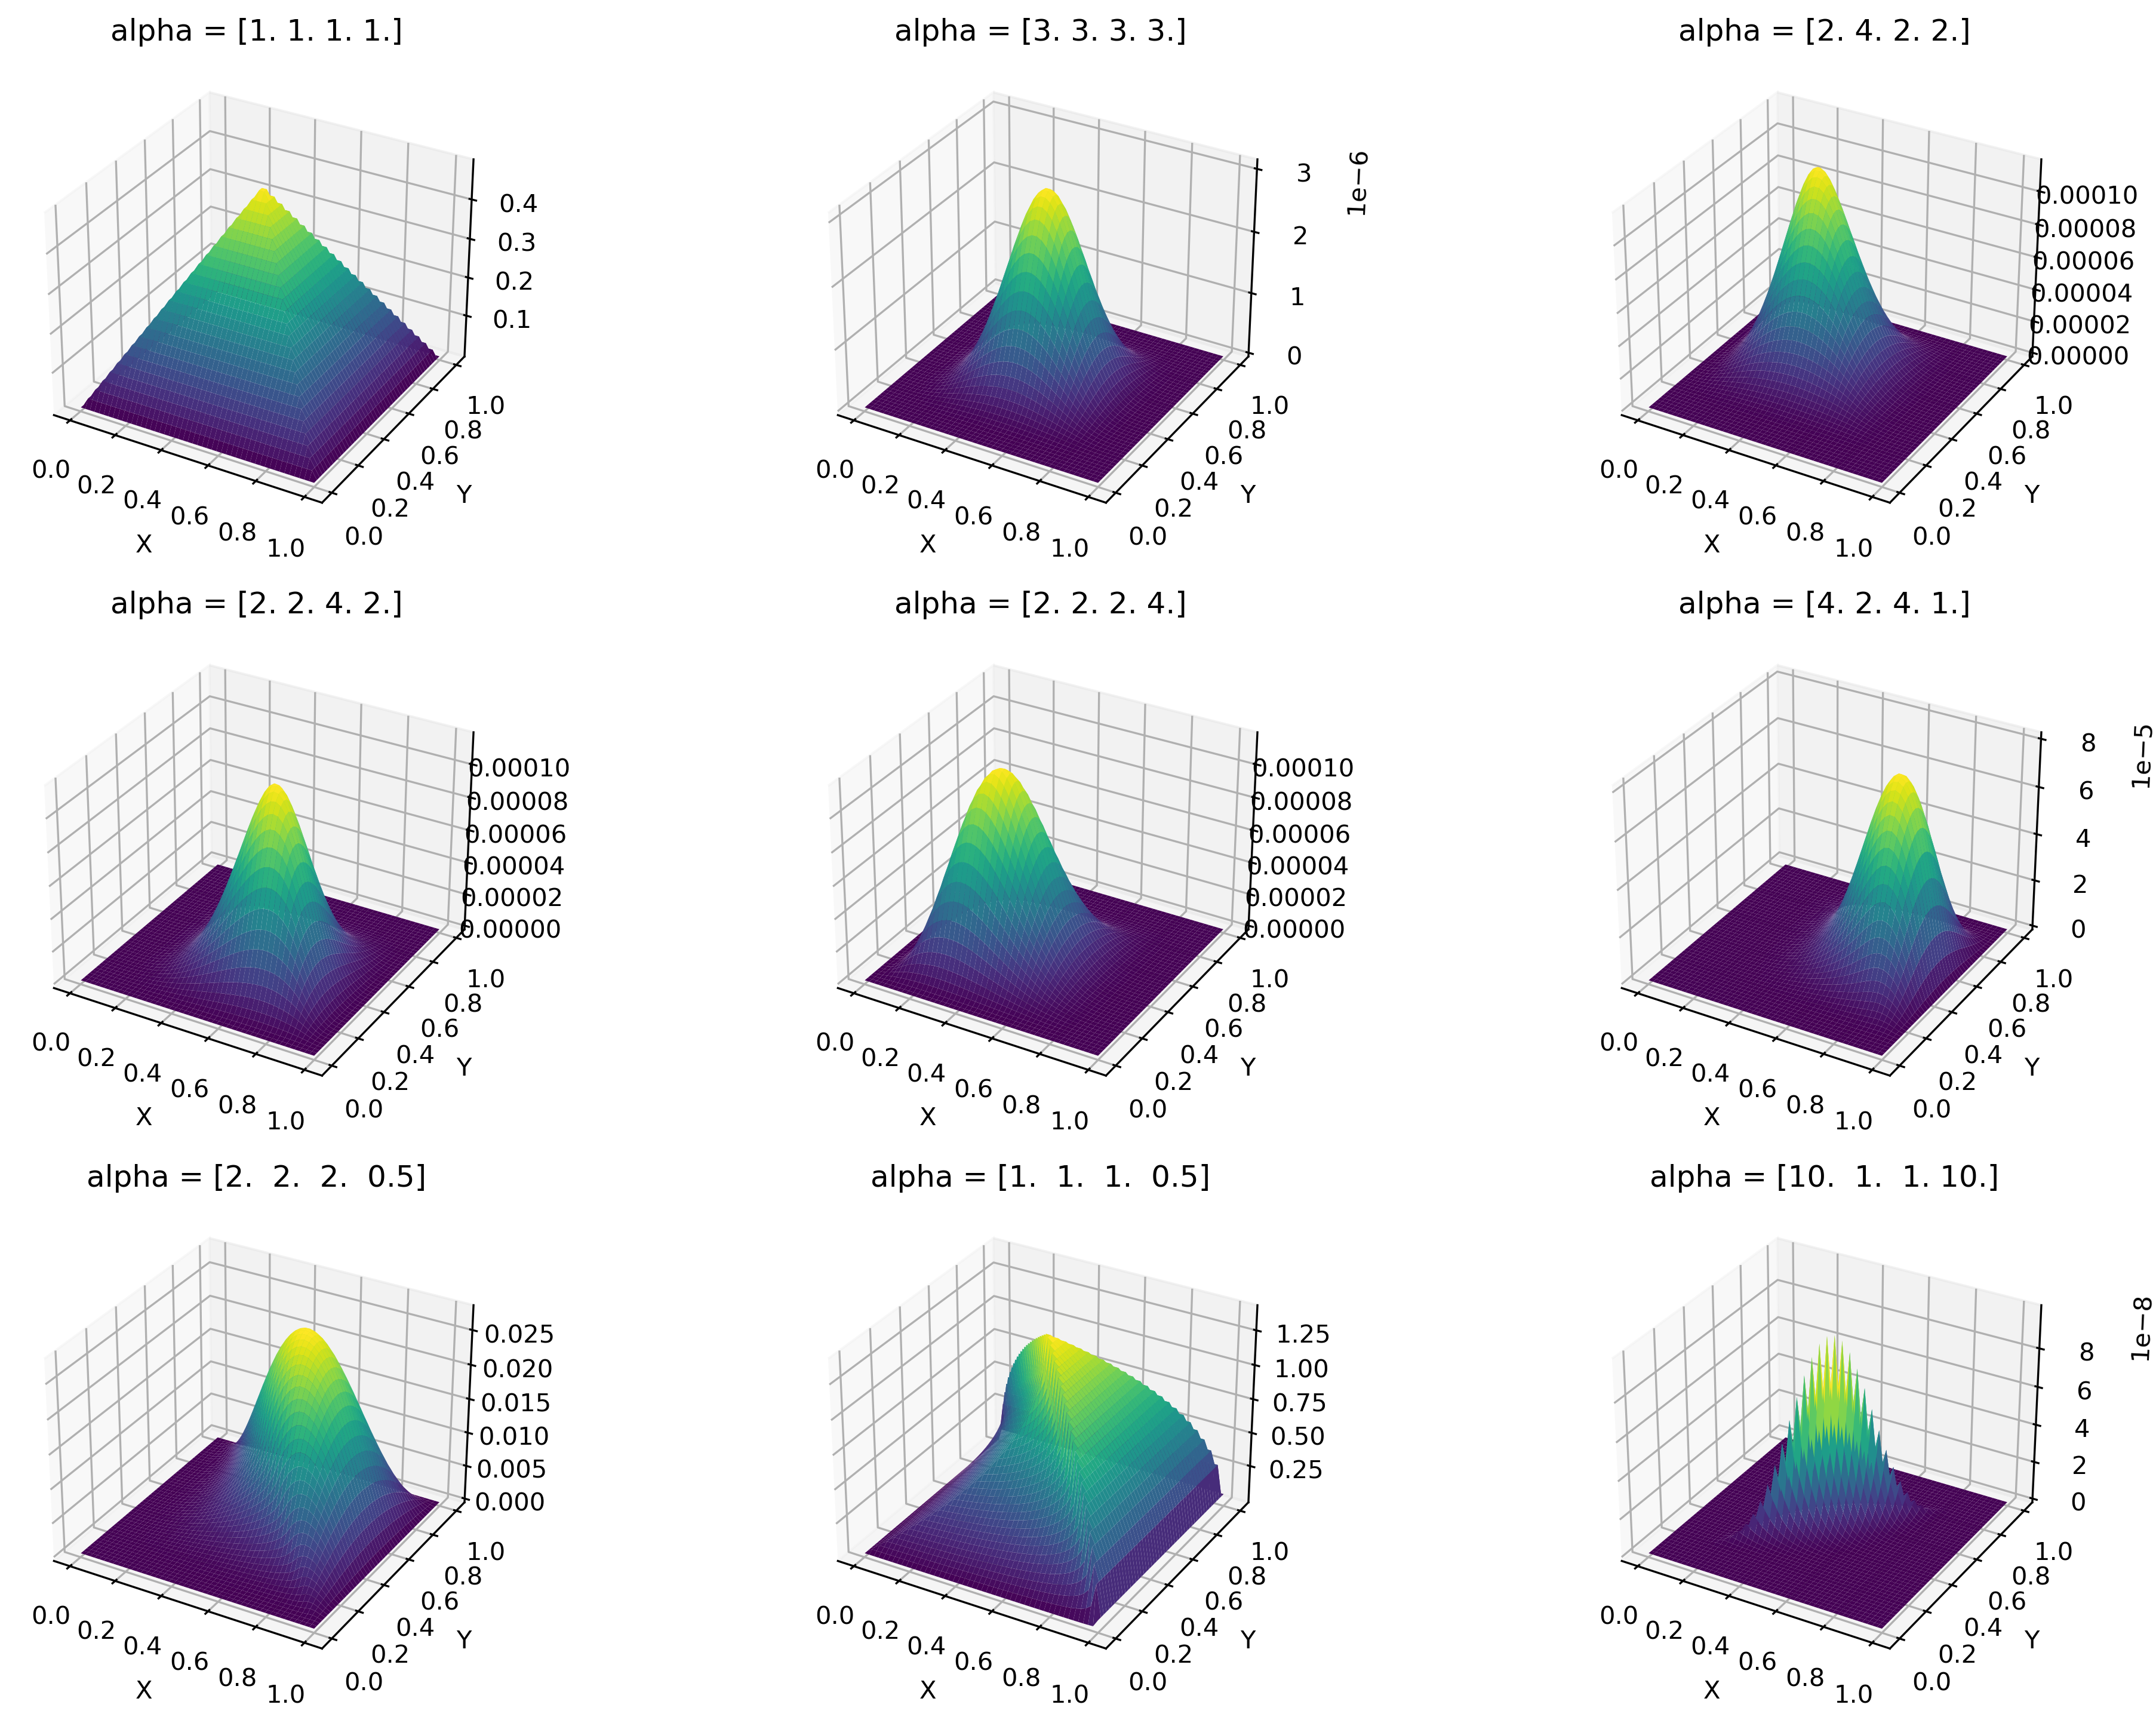
\includegraphics[width=\textwidth]{beta-distributions.png}
    \caption{Different choices of $\alpha$ and the joint distribution of the variables $X$ and $Y$.}
    \label{fig:beta-bivariate}
\end{figure}

In this section, we shall describe how to use the Bivariate Beta (see Appendix
\ref{appendix:bivariate-beta-distribution}) to model the correlation between
specificity and sensitivity.

\section{Imperfect tests}

This model includes the sensitivity and specificity of the diagnostic test. 

\begin{equation}
  \begin{aligned}
    T_i &\sim \bern(p_i) \\
    p_i &= \gamma_s\theta_i + (1-\gamma_e)(1 - \theta_i),  \\
    g(\theta_i) &= g(\theta) + \x_i^T\beta,  \\
    \beta &\sim \N(\mu, \Sigma), \\ 
    \theta &\sim \betadist(a^p, b^p) \\
    \gamma_s &\sim \betadist(a^s, b^s), \\
    \gamma_e &\sim \betadist(a^e, b^e), \\    
  \end{aligned}  
\end{equation}
where $a^p, a^s, a^e, b^p, b^s, b^e \in \R_{++}$ are fixed hyperparameters.
This model does not include prior knowledge about the correlation between
specificity and sensitivity. 

\subsection{Toy example}

Consider the following model \cite{gelman2020bayesian}:
\begin{gather*}
  y \sim \operatorname{Binomial}(n, p), \\
  p = \theta\gamma_s + (1- \theta)(1-\gamma_e), 
\end{gather*}
such that $y$ is the number of positive tests in a population of size $n$. In
a Bayesian paradigm, a prior $\pi(\theta, \gamma_e, \gamma_s)$ must be
specified. For instance, $\pi(\theta, \gamma_e, \gamma_s) =
\pi(\theta)\pi(\gamma_e, \gamma_s)$ and $\theta \sim
\operatorname{Beta}(\alpha_{\theta}, \beta_{\theta})$, in which
$\alpha_{\theta}$ and $\beta_{\theta}$ are positive hyperparameters. Since the
three parameters $\theta, \gamma_e$, and $\gamma_s$ are not jointly
identifiable only from $y$, prior information on $\gamma_e$ and $\gamma_s$
need be added. 

\section{Imperfect tests and respondent-driven sampling}

For now, we consider the network dependence induced by the RDS with no
associated model. Therefore, we treat it as a random effect for
each individual. Conditionally autoregressive (CAR) models in the
Gaussian case are used. Let $[\tilde{Q}]_{ij} = \tilde{q}_{ij}$ be a fixed matrix which measures the distance between $i$
and $j$, and $\tilde{q}_{i+} = \sum_{j} \tilde{q}_{ij}$. In general, we use
$$
\tilde{q}_{ij} = \begin{cases}
  1, &\text{if } i \text{ recruited } j \text{ or the contrary} \\
  0, &\text{otherwise.} 
\end{cases}
$$
Next we define the scaled adjacency matrix $Q = D^{-1}\tilde{Q}$, such that $D$
is a diagonal matrix with $D_{ii} = \tilde{q}_{i+}$. Finally let $|\rho| < 1$ be a
parameter to controls the dependence between neighbors. Hence, we specify the
model as follows:

\begin{equation}
  \begin{aligned}
    T_i &\sim \bern(p_i) \\
    p_i &= \gamma_s\theta_i + (1-\gamma_e)(1 - \theta_i),  \\
    g(\theta_i) &= g(\theta) + \x_i^T\beta + \omega_i,  \\
    \omega_i|\{\omega_j\}_{j\neq i}, \tau &\sim \N\left(\rho\sum_j q_{ij}\omega_j, \tau^{-1}/\tilde{q}_{i+}\right) \\
    \beta &\sim \N(\mu, \Sigma), \\ 
    \theta &\sim \betadist(a^p, b^p) \\
    \gamma_s &\sim \betadist(a^s, b^s), \\
    \gamma_e &\sim \betadist(a^e, b^e), \\  
    \tau &\sim \operatorname{Gamma}(a^{\tau}, b^{\tau}).
  \end{aligned}  
\end{equation}
By Brook's Lemma \cite[]{brook1964distinction}, the joint distribution of
$\omega$ can be specified as 
$$
\omega \sim \N\left(0, \left[\tau (D - \rho \tilde{Q})\right]^{-1}\right).
$$

\subsection{Toy example}

\begin{enumerate}
  \item Between the model with the log odds of prevalence having a Gaussian prior
  distribution and the other with the prevalence having a Beta prior
  distribution, 
  the latter was usually faster and without divergences. Therefore the 
  preferable model is with the prevalence. 

  \item Non-centered distributions are really worst. 
  \item Comparison between parametrization of sigma and tau showed that
  they are similar in sight of time of execution, energy and divergences,
  among others diagnostics. However, the mean estimate of sigma is more
  controlled. The median estimate is very similar. This happens because there
  are a few very high samples for $\tau$ that will have high weight in the
  final result. Small samples for $\sigma$ have less impact, despite having
  some. 
  \item More sparse matrices (RDS data is very sparse) is generating the funil
  we do not want to see. This is not connected to the number of connected
  components. In order to see that, a simple example with the Erdos-Renyi
  Random Graph can answer to us. In the sparse case, the number of edges is
  $O(n)$ with $p=1/n$. If $p=1$, the number of edges is $O(n^2)$ and the funil
  disappears. This problem does not appear in the poisson model. 

  \item The effect of $\rho$ is really observed in the literature in the
  paper: ``A close look at the spatial structure implied by the CAR and SAR
  models''. 
\end{enumerate}

\subsection{Exponential Random Graph Model (ERGM)}

RDS has the constraint of being without replacement. For that reason, we do
not observe all links among the samples \cite[]{crawford2016}. Considering the
model developed by Crawford, we can model the
matrix $Q$ as {\em Exponential Random Graph Model} (ERGM). Define the
following 

\begin{enumerate}
  \item $\boldsymbol{s} = \tril(QC)^T \boldsymbol{1} + C^Tu$, such that $Q$ is the
  adjacency matrix of the recruited subjects, $C$ is the {\em Coupon Matrix},
  $u$ the vector of the number of edge ends belonging to each vertex
  (in the order of recruitment) that are not connected to any other sampled
  vertex, and $\tril(M)$ the lower triangle of $M$. 

  \item $T(Q) = -\lambda \boldsymbol{s}$, such that $\lambda$ is the rate of
  the recruitment time. 

  \item $V(Q) = \sum_{k \text{ is not seed}} \log(\lambda \boldsymbol{s}_k)$
  
  \item $w = (0, t_2 - t_1, ..., t_n - t_{n-1})$ is the vector of the waiting times between
  recruitments.  
\end{enumerate}

Therefore $\Pr(Q|w) \propto \exp[T(Q)^Tw + V(Q)]$. With that, the model
becomes 

\begin{equation}
  \begin{aligned}
    T_i &\sim \bern(p_i) \\
    p_i &= \gamma_s\theta_i + (1-\gamma_e)(1 - \theta_i),  \\
    g(\theta_i) &= g(\theta) + \x_i^T\beta + \omega_i,  \\
    \omega_i|\{\omega_j\}_{j\neq i}, \tau &\sim \N\left(\rho\sum_j q_{ij}\omega_j/q_{i+}, \tau^2/q_{i+}\right) \\
    Q|w &\propto \exp[T(Q)^Tw + V(Q)] \\
    \lambda &\sim \Gamma(a^{\lambda}, b^{\lambda}), \\ 
    \beta &\sim \N(\mu, \Sigma), \\ 
    \theta &\sim \betadist(a^p, b^p) \\
    \gamma_s &\sim \betadist(a^s, b^s), \\
    \gamma_e &\sim \betadist(a^e, b^e), \\  
    \tau &\sim \N^+(0,\sigma^2_{\tau}).
  \end{aligned}  
\end{equation}
The problem with this model is that we are assigning a posterior distribution
for $Q$.